\section{Bonus: M\"obius inversion on partially ordered sets}
\label{sec:poset-inversion}

For ordinary running totals $G(j)=F(0)+\cdots+F(j)$, subtraction
recovers $F(j)=G(j)-G(j-1)$ for $j\ge1$, with $F(0)=G(0)$.
Divisor sums have a more complicated inverse because divisibility
branches: $2$ and $3$ both precede $6$, but neither precedes the other.
We can describe the common operation as adding all contributions
below a given object in an order.

\subsection{Orders, intervals, and diagrams}

A \emph{partial order} $\le$ on a set $P$ is reflexive
($x\le x$), antisymmetric ($x\le y$ and $y\le x$ imply $x=y$),
and transitive. The pair is a \emph{partially ordered set}, or
\emph{poset}. Two elements need not be comparable.
Examples are integers in their usual order, positive divisors of
an integer ordered by divisibility, and subsets of a set ordered
by inclusion. The symbol $\le$ below always means the chosen order.

The \emph{interval} $[x,y]$ is $\{z:x\le z\le y\}$.
In a \emph{Hasse diagram}, larger elements appear higher; join $x$
to $y$ when $x<y$ and there is no element strictly between them.
Transitive comparisons are represented by upward paths.

\begin{center}
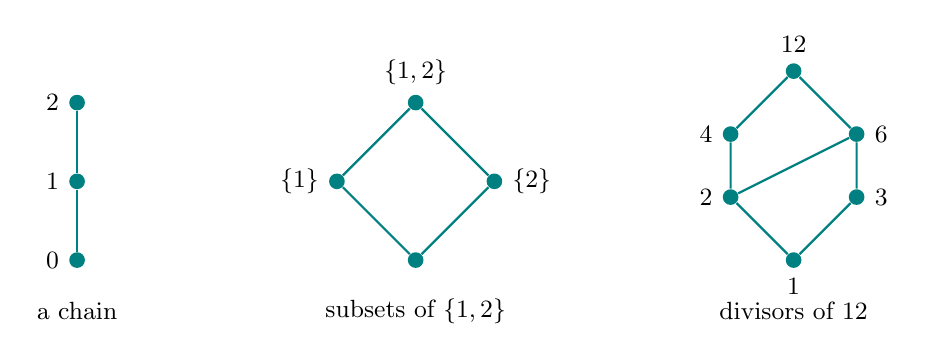
\begin{tikzpicture}[every node/.style={font=\small},
 dot/.style={circle,fill=teal,inner sep=2pt}]
 \begin{scope}
  \node[dot,label=left:$0$] (c0) at (0,0) {};
  \node[dot,label=left:$1$] (c1) at (0,1) {};
  \node[dot,label=left:$2$] (c2) at (0,2) {};
  \draw[teal,thick] (c0)--(c1)--(c2);
  \node at (0,-.65) {a chain};
 \end{scope}
 \begin{scope}[xshift=4.3cm]
  \node[dot,label=below:$\varnothing$] (b0) at (0,0) {};
  \node[dot,label=left:$\{1\}$] (b1) at (-1,1) {};
  \node[dot,label=right:$\{2\}$] (b2) at (1,1) {};
  \node[dot,label={above:$\{1,2\}$}] (b3) at (0,2) {};
  \draw[teal,thick] (b0)--(b1)--(b3)--(b2)--(b0);
  \node at (0,-.65) {subsets of $\{1,2\}$};
 \end{scope}
 \begin{scope}[xshift=9.1cm]
  \node[dot,label=below:$1$] (d1) at (0,0) {};
  \node[dot,label=left:$2$] (d2) at (-.8,.8) {};
  \node[dot,label=right:$3$] (d3) at (.8,.8) {};
  \node[dot,label=left:$4$] (d4) at (-.8,1.6) {};
  \node[dot,label=right:$6$] (d6) at (.8,1.6) {};
  \node[dot,label=above:$12$] (d12) at (0,2.4) {};
  \draw[teal,thick] (d1)--(d2)--(d4)--(d12)--(d6)--(d3)--(d1);
  \draw[teal,thick] (d2)--(d6);
  \node at (0,-.65) {divisors of $12$};
 \end{scope}
\end{tikzpicture}
\end{center}

For now assume $P$ is finite. Given exact contributions $F(x)$, define
the cumulative values $G(y)=\sum_{x\le y}F(x)$. We can always recover
$F(y)=G(y)-\sum_{x<y}F(x)$, starting with minimal elements.
The inverse therefore exists and is unique. Its coefficients depend
only on the order, not on the values being added.

\subsection{Define the inverse by cancellation}

\begin{definition}
For comparable elements of a finite poset, define its
\emph{M\"obius function} recursively by
\[
 \mu_P(x,x)=1,\qquad
 \mu_P(x,y)=-\sum_{x\le z<y}\mu_P(x,z)\quad(x<y).
\]
Equivalently,
$\sum_{x\le z\le y}\mu_P(x,z)=\delta_{xy}$, where
$\delta_{xy}$ is $1$ if $x=y$ and $0$ otherwise.
\end{definition}

\begin{theorem}[M\"obius inversion on a finite poset]
For functions $F,G:P\to\R$,
\[
 G(y)=\sum_{x\le y}F(x)\quad\text{for all }y
 \quad\Longleftrightarrow\quad
 F(y)=\sum_{x\le y}\mu_P(x,y)G(x)\quad\text{for all }y.
\]
\end{theorem}
\begin{proof}
Let $H(y)$ denote the proposed inverse on the right. Its cumulative
sum is
\[
 \begin{aligned}
 \sum_{y\le t}H(y)
 &=\sum_{y\le t}\sum_{x\le y}\mu_P(x,y)G(x)\\
 &=\sum_{x\le t}G(x)\sum_{x\le y\le t}\mu_P(x,y)=G(t).
 \end{aligned}
\]
Thus $H$ has cumulative values $G$. Successive subtraction gives
a unique such function, so $H=F$. This calculation also proves the
reverse implication.
\end{proof}

There is an equally useful form for totals \emph{above} an element:
\[
 G(x)=\sum_{y\ge x}F(y)
 \quad\Longleftrightarrow\quad
 F(x)=\sum_{y\ge x}\mu_P(x,y)G(y).
\]
To verify the inverse, substitute the upper sum for $G(y)$ and collect
the coefficient of $F(z)$; it is
$\sum_{x\le y\le z}\mu_P(x,y)=\delta_{xz}$.
Successive subtraction from maximal elements proves uniqueness.

\subsection{Three familiar inversions}

\textbf{A chain gives finite differences.}
On $0<1<\cdots<N$, the recurrence gives
\[
 \mu_P(i,j)=
 \begin{cases}
 1,&j=i,\\
 -1,&j=i+1,\\
 0,&j\ge i+2.
 \end{cases}
\]
The first two terms cancel in every longer interval, so all later
terms are zero. The theorem recovers ordinary subtraction of running totals.

\textbf{Divisibility gives arithmetic M\"obius inversion.}
If $r\mid s$, the elements of $[r,s]$ correspond to divisors of $s/r$
by $t\mapsto t/r$. The arithmetic cancellation lemma gives
\[
 \sum_{r\mid t\mid s}\mu(t/r)=\varepsilon(s/r)=\delta_{rs}.
\]
Uniqueness in the recursive definition therefore gives
$\mu_P(r,s)=\mu(s/r)$. The poset theorem becomes precisely the
divisor-sum formula from Section~\ref{sec:mobius-inversion}.

\textbf{Subset inclusion gives inclusion--exclusion.}
For subsets $S\subseteq T$ of a fixed finite set,
\[
 \mu_P(S,T)=(-1)^{|T\setminus S|}.
\]
To check the recurrence, sum $(-1)^{|U\setminus S|}$ over
$S\subseteq U\subseteq T$. If $S\ne T$, choose an element of
$T\setminus S$ and pair subsets by inserting or removing it.
The signs cancel; for $S=T$, the sum is $1$.
Thus
\[
 G(T)=\sum_{S\subseteq T}F(S)
 \quad\Longleftrightarrow\quad
 F(T)=\sum_{S\subseteq T}(-1)^{|T\setminus S|}G(S).
\]

To see the usual counting formula, let $A_1,\ldots,A_r$ be subsets
of a finite universe $U$. Let $F(T)$ count elements whose set of
memberships is \emph{exactly} $T$, and put
$G(S)=|\bigcap_{i\in S}A_i|$, with $G(\varnothing)=|U|$.
Then $G(S)=\sum_{T\supseteq S}F(T)$: an intersection allows
additional memberships. Apply the \emph{upper} version of inversion
at the empty set:
\[
 \left|U\setminus\bigcup_{i=1}^r A_i\right|
 =\sum_{S\subseteq\{1,\ldots,r\}}(-1)^{|S|}
   \left|\bigcap_{i\in S}A_i\right|.
\]
Subtract from $|U|$ to obtain the usual alternating formula for the union.

\subsection{A coefficient larger than one: partitions}

A partition divides a set into nonempty disjoint blocks.
Order partitions by \emph{refinement}: $\pi\le\sigma$ when every
block of $\pi$ lies inside a block of $\sigma$.
For $\{1,2,3\}$ there are five partitions:
\[
 \widehat0=1|2|3,\qquad 12|3,\ 13|2,\ 23|1,\qquad
 \widehat1=123.
\]
The three middle partitions are incomparable, each above $\widehat0$
and below $\widehat1$. The recursive coefficients from $\widehat0$
are $1$ at the bottom, $-1$ at each middle element, and
\[
 \mu_P(\widehat0,\widehat1)=-\bigl(1-1-1-1\bigr)=2.
\]
So poset M\"obius coefficients need not belong to $\{-1,0,1\}$.

Color the three labeled positions with $a$ colors. Let $F(\sigma)$
count colorings whose equality classes are exactly the blocks of
$\sigma$. Let $G(\pi)$ count colorings constant on every block of
$\pi$, allowing different blocks to receive the same color.
Then $G(\pi)=a^{b(\pi)}$, where $b(\pi)$ is its number of blocks,
and $G(\pi)=\sum_{\sigma\ge\pi}F(\sigma)$.
Upper inversion at $\widehat0$ gives the number with all colors distinct:
\[
 F(\widehat0)=a^3-3a^2+2a=a(a-1)(a-2).
\]
The coefficient $2$ corrects the three overlapping ways of merging
a pair. It is determined by the partition order.

\subsection{Independent orders multiply the coefficients}

The product poset $P\times Q$ has
$(x,u)\le(y,v)$ exactly when $x\le y$ and $u\le v$.
Its M\"obius function factors:
\[
 \mu_{P\times Q}((x,u),(y,v))=\mu_P(x,y)\mu_Q(u,v).
\]
Indeed, summing the proposed coefficients over the product interval
factors as
\[
 \left(\sum_{x\le z\le y}\mu_P(x,z)\right)
 \left(\sum_{u\le w\le v}\mu_Q(u,w)\right)
 =\delta_{xy}\delta_{uv}.
\]
This is the defining cancellation rule, so uniqueness proves the claim.

The divisors of $n=\prod_i p_i^{k_i}$ form the product of exponent
chains $0<1<\cdots<k_i$. A jump of two or more steps in any chain
has coefficient zero. This explains structurally why $\mu(n)$
vanishes when a prime square divides $n$, and otherwise equals one
factor of $-1$ for each prime. Likewise, the subsets of an $r$-element
set form a product of $r$ two-element chains, explaining the signs
in inclusion--exclusion.

\subsection{The algebra behind the cancellation}

For functions $A,B$ on comparable pairs of a finite poset, define
\[
 (A*B)(x,y)=\sum_{x\le z\le y}A(x,z)B(z,y).
\]
These functions, with pointwise addition and this convolution, form
the \emph{incidence algebra}. The identity is $\delta(x,y)=\delta_{xy}$;
associativity follows by summing over $x\le z\le w\le y$.
The \emph{zeta function} is $\zeta(x,y)=1$ for $x\le y$.
The recurrence and inversion theorem say
\[
 \mu_P*\zeta=\zeta*\mu_P=\delta.
\]
If the elements are listed so that smaller ones precede larger ones,
these are upper triangular matrices: zeta performs cumulative summation
and its inverse supplies the M\"obius coefficients.

On positive integers ordered by divisibility, the pair function
$A_f(r,s)=f(s/r)$ satisfies
\[
 (A_f*A_g)(r,s)=\sum_{r\mid t\mid s} f(t/r)g(s/t)
              =(f*g)(s/r).
\]
Dirichlet convolution is therefore this incidence convolution for
functions depending only on the quotient of the endpoints.

\begin{warningbox}[breakable=false]
An infinite poset is \emph{locally finite} when each interval $[x,y]$
is finite. That suffices to define the incidence algebra and its
M\"obius function. For sums over \emph{all} $x\le y$, also require
finitely many contributing terms, for example finite lower sets or
finitely supported data. Local finiteness alone does not ensure this:
the usual order on $\Z$ has finite intervals but infinitely many
elements below each integer. All examples computed here use finite sums.
\end{warningbox}

\begin{bigidea}
First identify what ``exactly'' means and what the cumulative count
includes. Then choose the order connecting those two counts.
Divisibility leads to arithmetic M\"obius inversion, inclusion to
inclusion--exclusion, and refinement to partition coefficients.
In each case the inverse cancels all unwanted intermediate contributions.
\end{bigidea}
